\chapter{Perancangan Sistem}

\section{Alur Perancangan}
\begin{figure}[h]
	\centering
	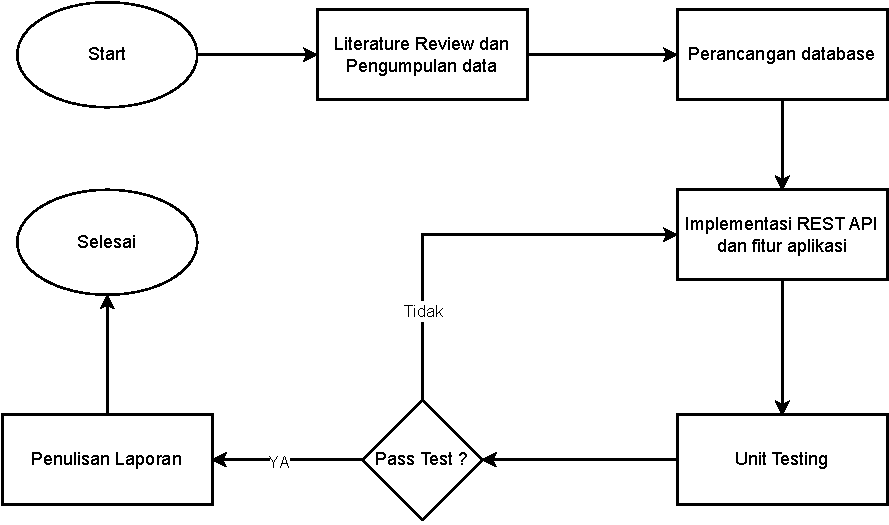
\includegraphics[width=0.75\textwidth]{drawio/alur-perancangan.drawio.pdf}
	\caption{Alur Perancangan}
	\label{alur-perancangan}
\end{figure}
Gambar \ref{alur-perancangan} menunjukkan alur perancangan sistem \textit{backend} yang dibuat. Terdapat 5 tahapan dalam perancangan sistem yaitu :

\subsection{\textit{Literature Review} dan Pengumpulan data}
Pada tahap ini, dilakukan pengumpulan data melalui Software Requirement Specification (SRS) yang telah dibuat oleh System Analyst (SA) serta membaca literatur ilmiah mengenai pengembangan \textit{backend} web.

\subsection{Perancangan database}
Pada tahap ini dilakukan perancangan dan implementasi ERD menggunakan PrismaJs sebagai \textit{framework} Object Relational Mapping.

\subsection{Implementasi REST API dan fitur aplikasi}
Pada tahap ini dilakukan sesi koding untuk mengimplementasikan berbagai macam fitur aplikasi berdasarkan SRS yang telah dibuat dan membuat API \textit{endpoint} yang menghindari \textit{anti pattern}.

\subsection{Unit Testing}
Pada tahap unit testing, dilakukan pengujian logic dan fungsi API, sampai tidak terdapat error lagi, maka dilanjut ke penulisan proposal.

\subsection{Penulisan laporan}
Pada tahap ini, akan disusun semua tahapan pekerjaan, hasil analisis dan pembahasan terhadap semua yang telah dilakukan, diamati, dan dihasilkan dalam membuat dan mengimplementasikan \textit{backend} aplikasi.

\section{Desain Sistem}
\begin{figure}[h]
	\centering
	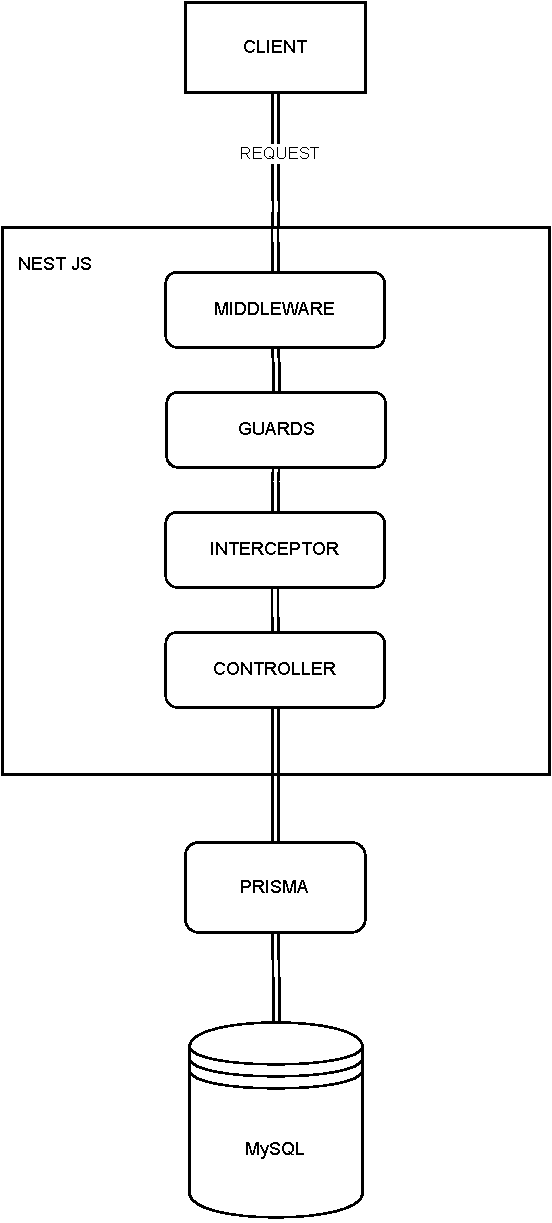
\includegraphics[width=0.35\textwidth]{drawio/sistem-desain.drawio.pdf}
	\caption{Desain Sistem}
	\label{sistem-desain}
\end{figure}
Implementasi dan perancangan RESTful API, Database, dan fungsi bisnis dikembangkan menggunakan \textit{framework} NestJs. Pada NestJs terdapat beberapa komponen seperti: Middleware, Guards, Interceptor, Controller, dan Service. Service yang dipakai adalah PrismaJs untuk menghubungkan NestJs ke \textit{Database System}. Gambar \ref{sistem-desain} merupakan \textit{Request Lifecycle} yang menjelaskan bagaimana alur \textit{request} ditangani dari awal sampai akhir.
Pada Middleware, fungsi akan dipanggil sebelum masuk ke routing. Pada Guard, \textit{request} akan dicek \textit{authenticity}, untuk mengetahui validitas dari \textit{request} tersebut. Tahap ini juga akan dicek keamanan session menggunakan JWT dan CSRF. Setelah melalui Guard, Request akan masuk ke Interceptor. Dimana jika suatu \textit{request} mempunyai suatu karakteristik yang ditentukan, maka akan menjalankan fungsi tambahan. Interceptor terjadi ketika \textit{request} datang \textit{(pre)}, dan response \textit{(post)}. Setelah melewati Interceptor, fungsi di Controller akan dijalankan. Jika pada Controller tersebut perlu data dari database maka akan turun ke service PrismaJs untuk melakukan database call menggunakan ORM \cite{NestJS}.

\begin{figure}[h]
	{\centering {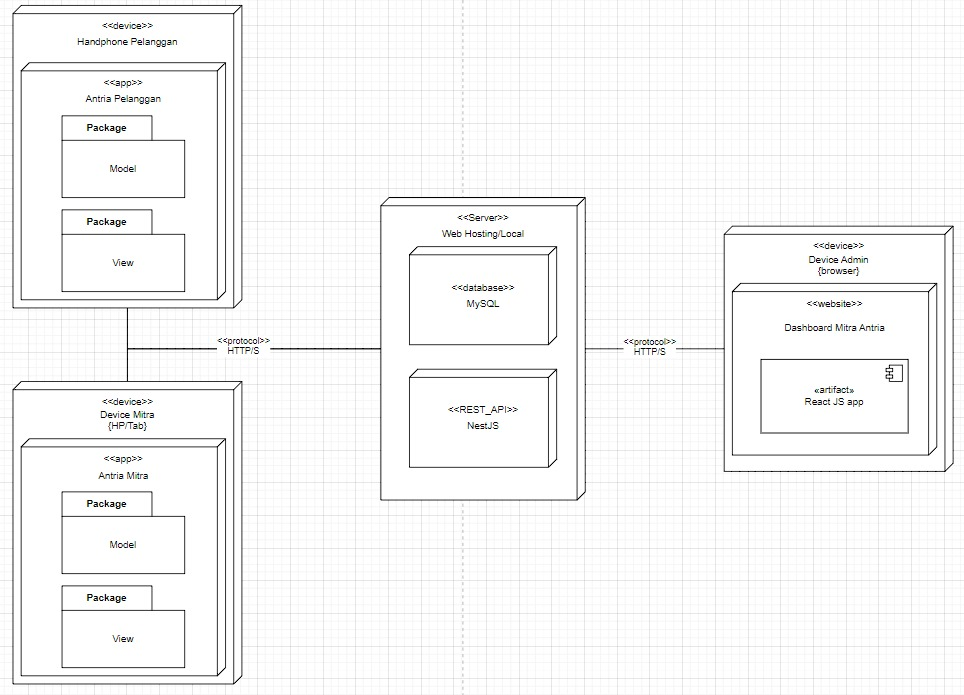
\includegraphics[scale=0.5]{drawio/deployment.jpg}}\par}
	\caption{Deployment Diagram}
	\label{deployment}
\end{figure}
Pada diagram \ref{deployment} menjelaskan bagaimana server backend berkomunikasi dengan Aplikasi lain melalui protokol HTTPS. 

